\documentclass[10pt, titlepage, oneside, a4paper]{article}
\usepackage[T1]{fontenc}
\usepackage[utf8]{inputenc}
\usepackage[swedish]{babel}
\usepackage{amssymb, graphicx, fancyhdr}
\usepackage{hyperref}
\usepackage{pgf, tikz}
\usepackage{pgfplots}
\usepackage{listings}
\usepackage{color}
\usepackage{amsmath}
\usepackage{mathtools}
\usepackage{float}
\addtolength{\textheight}{20mm}
\addtolength{\voffset}{-5mm}
\renewcommand{\sectionmark}[1]{\markleft{#1}}

\newcommand{\Section}[1]{\section{#1}\vspace{-8pt}}
\newcommand{\Subsection}[1]{\vspace{-4pt}\subsection{#1}\vspace{-8pt}}
\newcommand{\Subsubsection}[1]{\vspace{-4pt}\subsubsection{#1}\vspace{-8pt}}


\def\typeofdoc{Laborationsrapport}
\def\course{F0004T}
\def\pretitle{Laboration 1}
\def\title{Svängningstid av svängande svängningar}
\def\username{magbjr-3}
\def\domain{@student.ltu.se}
\def\email{\username{}@student.ltu.se}
\def\group{Grupp 10}
\def\graders{Magnus Frediksson}
\def\university{Luleå Tekniska Universitet}


\def\fullpath{\raisebox{1pt}{$\scriptstyle \sim$}\username/\path}


\begin{document}
	\begin{titlepage}
		\thispagestyle{empty}
		\begin{large}
			\begin{tabular}{@{}p{\textwidth}@{}}
				\textbf{\university\hfill\today}\\
				\textbf{\typeofdoc} \\
			\end{tabular}
		\end{large}
		\vspace{10mm}
		\begin{center}
			\LARGE{\pretitle} \\
			\huge{\textbf{\course}}\\
			\vspace{10mm}
			\LARGE{\title}\\
			\vspace{15mm}
			\begin{large}
				\begin{tabular}{l|ll}
                    \textbf{\group} & \textbf{Namn} & \textbf{E-mail}\\
                    \hline
                    & \texttt{Anton Eriksson}   & \texttt{eriano-4\domain}       \\
                    & \texttt{Eric Öhman}   & \texttt{erihma-3\domain}       \\
                    & \texttt{Magnus Björk}   & \texttt{magbjr-3\domain}       \\
				\end{tabular}
			\end{large}
			\vfill
			\large{\textbf{Handledare}}\\
			\mbox{\large{\graders}}
		\end{center}
	\end{titlepage}


	\lfoot{\footnotesize{\group}}
	\rfoot{\footnotesize{\today}}
	\lhead{\sc\footnotesize\title}
	\rhead{\nouppercase{\sc\footnotesize\leftmark}}
	\pagestyle{fancy}
	\renewcommand{\headrulewidth}{0.2pt}
	\renewcommand{\footrulewidth}{0.2pt}

	\pagenumbering{roman}
    \begin{abstract}
    \end{abstract}
    
    \tableofcontents
	
	\newpage
	\pagenumbering{arabic}

	\setlength{\parindent}{10pt}
	\setlength{\parskip}{10pt}
    
	\section{Inledning}
	\section{Metod}
    För att strukturera arbetet gjordes en planering av laborationen. Detta görs enligt en standardiserad metod som är vanlig i projekt som detta där samband ska tas fram.
    \begin{enumerate}
        \item Deifiniera Problemet.
        \item Vad påverkar?
        \item Planera mätningar.
        \item Resultat Tabell.
        \item Rita Figurer.
        \item Analysera (Linjärisera).
        \item Dimensionsanalys.
    \end{enumerate}

Materialen som användes i laborationen: Ställning för balkar, fotocell, dosa för avläsning av fotocellens mätningar, balkar i fyra olika material samt olika dimensioner, måttband.

 Fyra olika tester genomfördes för att kunna ta fram sambandet mellan period tiden och ändringen i längd, tjocklek, bredd och material.
Mätningarna utfördes genom att man fäste balken som skulle testas i ställningen. Balken fästes bara i ena änden medans den andra änden var fri och kunde röra sig i vertikalled. I den fria änden placerades fotocellen för att kunna mäta balkens svängningstid. Fotocellen placerades så nära balkens ände som möjligt för att   I första testet användes endast en stålbalk. Det enda som ändrades i detta test var längden på balken.
    \section{Analys}
        \subsection{Variabellista}
        \begin{table}[h]
            \begin{tabular}{llll}

            \textbf{Storhet} & \textbf{Symbol} & \textbf{Enhet} & \textbf{Grunddimension} \\ \hline
            Pendeltid    & T    & s     & T         \\ \hline
            Balklängd    & l    & m     & L         \\ \hline
            Balktjocklek & h    & m     & L         \\ \hline
            Balkbredd    & b    & m     & L         \\ \hline
            Densitet     & $\rho$    & $kg/m^3$ & $M\cdot L^{-3}$     \\ \hline
            E-modul      & E      & \footnotesize $kg/ms^2$    &                \\ \hline
            \end{tabular}
        \end{table} 
        
	\section{Resultat}
    \begin{figure}[H]
        \centering
        \includegraphics[scale=.5]{../png/height.png}
        \caption{Svängningstid beroende på tjocklek.}
        \label{height}
    \end{figure}

    \begin{table}[H]
        \caption{Undersökning av tjocklek.}
        \begin{center}
            \begin{tabular}{cccc}
                \hline
                Tid (s) & Längd (m) & Tjocklek (m) & Bredd (m)\\
                \hline
                0.421 & 1.000 & 0.003 & 0.020\\
                0.254 & 1.000 & 0.005 & 0.020\\
                0.215 & 1.000 & 0.006 & 0.020\\
                0.162 & 1.000 & 0.008 & 0.020\\
            \end{tabular}
        \end{center}
    \end{table}

    \begin{figure}[H]
        \centering
        \includegraphics[scale=.5]{../png/length.png}
        \caption{Svängningstid beroende på längd.}
        \label{length}
    \end{figure}
    \begin{table}[H]
        \caption{Undersökning av längd.}
        \begin{center}
            \begin{tabular}{cccc}
                \hline
                Tid (s) & Längd (m) & Tjocklek (m) & Bredd (m)\\
                \hline
                0.362 & 1.200 & 0.005 & 0.020\\
                0.305 & 1.100 & 0.005 & 0.020\\
                0.254 & 1.000 & 0.005 & 0.020\\
                0.207 & 0.900 & 0.005 & 0.020\\
                0.164 & 0.800 & 0.005 & 0.020\\
                0.145 & 0.750 & 0.005 & 0.020\\
                0.094 & 0.600 & 0.005 & 0.020\\
                0.066 & 0.500 & 0.005 & 0.020\\
                0.083 & 0.400 & 0.005 & 0.020\\
            \end{tabular}
        \end{center}
    \end{table}
    \begin{figure}[H]
        \centering
        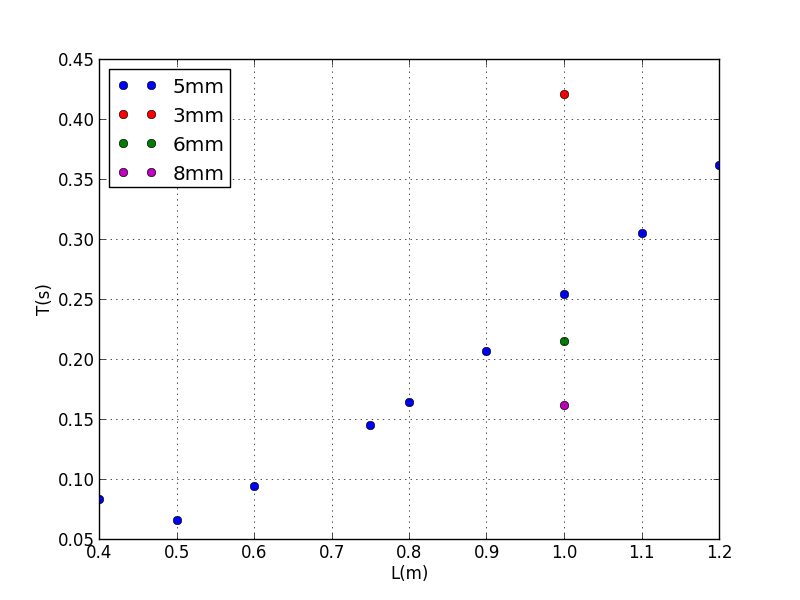
\includegraphics[scale=.5]{../png/plot.png}
        \caption{Svängningstid beroende på material.}
        \label{material}
    \end{figure}
    \begin{figure}[H]
        \centering
        \includegraphics[scale=.5]{../png/ln_t_ln_l.png}
        \caption{linearisering}
        \label{linearisering}
    \end{figure}


    \begin{table}
        \caption{Undersökning av bredd.}
        \begin{center}
            \begin{tabular}{cccc}
                \hline
                Tid (s) & Längd (m) & Tjocklek (m) & Bredd (m)\\
                \hline
                0.255 & 1.000 & 0.005 & 0.020\\
                0.259 & 1.000 & 0.005 & 0.025\\
                0.250 & 1.000 & 0.005 & 0.030\\
                0.259 & 1.000 & 0.005 & 0.040\\
            \end{tabular}
        \end{center}
    \end{table}

    \section{Diskussion}


\end{document}

